[129 r\textsuperscript{o}] \textso{Exper. Florent. de }\textso{press. aeris }\protect\index{Sachverzeichnis}{pressio!aeris} p. 31. habetur Mixtura occludendi  commissuras vitrorum, ne aer penetret. \selectlanguage{italian}Tal mestura se sara fatta  con polvere di matton pesto, ridotta per lungo macinamento impalpabile  e incorporata con trementina e pece greca sera attissima a stuccar  vetri, per modo, che l'aria di fuora ne resti esclusa.\selectlanguage{latin}\edtext{\edlabel{esc129r1}}{\lemma{esclusa.}\Bfootnote{\cite{00143}\textsc{L. Magalotti}, a.a.O., S.~XXXI.}}\pend 
\pstart \edtext{Vesicam flaccidam  in vacuo inflari primus\edlabel{esc129r2}}{\lemma{esclusa.}\xxref{esc129r1}{esc129r2}\Afootnote{ \textit{ (1) }\ Aquam primum \textit{ (2) }\ Vesicam  \textit{(a)}\ primum \textit{(b)}\ flaccidam  in  \textit{(aa)}\ aere \textit{(bb)}\ vacuo inflari primus \textit{ L}}} observavit Robervallius\protect\index{Namensregister}{\textso{Roberval} (Robervallius), Gilles Personne de 1602\textendash 1675}. Observatum  eandem manere altitudinem Mercurii\protect\index{Sachverzeichnis}{mercurius} etsi non liberi aeris pondus\protect\index{Sachverzeichnis}{pondus!aeris}  sed tantum Elater\protect\index{Sachverzeichnis}{elater} clausi ipsi opponatur. \edtext{In hac campana inclusum Barometrum}{\lemma{opponatur.}\Afootnote{ \textit{ (1) }\ Si in hac campana Mercurius\protect\index{Sachverzeichnis}{mercurius|textit} \textit{ (2) }\ In hac campana inclusum Barometrum \textit{ L}}} mutabat altitudinem, prout calore\protect\index{Sachverzeichnis}{calor}  aut frigore\protect\index{Sachverzeichnis}{frigor} mutabatur \edtext{Elater}{\lemma{mutabatur}\Afootnote{ \textit{ (1) }\ firmitas \textit{ (2) }\ Elater \textit{ L}}} aeris campanae. Et p. 62. fatentur Experimentum variantis Hydrargyri\protect\index{Sachverzeichnis}{hydrargyrus} pro altitudine locorum  primum in Francia\protect\index{Ortsregister}{Frankreich (Gallia, Francia)} repertum.\edtext{}{\lemma{repertum.}\Bfootnote{\cite{00143}\textsc{L. Magalotti}, a.a.O., S.~LXII.}} Et p. 68. \edtext{}{\lemma{68.}\Bfootnote{\cite{00143}\textsc{L. Magalotti}, a.a.O., S.~LXVIII.}} observatum calor\protect\index{Sachverzeichnis}{calor} in  imo et in summo turris Florentinae 142 brachiorum (vid. p. 64.\edtext{}{\lemma{64.}\Bfootnote{\cite{00143}\textsc{L. Magalotti}, a.a.O., S.~LXIV.}})  aequalis exacto thermometro\protect\index{Sachverzeichnis}{thermometrum} repertus esset, nihilominus [repertum]\edtext{}{\lemma{reperta}\Afootnote{\textit{\ L \"{a}ndert Hrsg. } }} vim aeris Elasticam\protect\index{Sachverzeichnis}{vis!elastica} in summo et in imo differentem.\pend \pstart  In Vacuo \textso{p. }[\textso{78}]\edtext{}{\Afootnote{\textso{68}\textit{\ L \"{a}ndert Hrsg. } }}.\edtext{}{\lemma{[\textso{78}].}\Bfootnote{\cite{00143}\textsc{L. Magalotti}, a.a.O., S.~LXXVIII.}} Guttae liquidorum non habent rotunditatem ab aeris pressione\protect\index{Sachverzeichnis}{pressio!aeris}, nam et retinent \edtext{aere  extracto}{\lemma{retinent}\Afootnote{ \textit{ (1) }\ aeris pressione\protect\index{Sachverzeichnis}{pressio!aeris|textit} e \textit{ (2) }\ aere  extracto \textit{ L}}}.\pend \pstart  P. 82. Keplerus\protect\index{Namensregister}{\textso{Kepler} (Keplerus), Johannes 1571\textendash 1630} in \textit{Astronomia Optica}, %\edtext{}{\lemma{\textit{Optica,}}\Bfootnote{\textsc{J. Kepler, }\cite{00195}\textit{Astronomiae pars optica}, Frankfurt 1604, S. ?.}} 
dixerat,  aerem folii loco servire superficiei posteriori lentis\protect\index{Sachverzeichnis}{lens} vitreae, et reflecti  inversam obscuriorem quam apparet a lumine\protect\index{Sachverzeichnis}{lumen} aut altero objecto  quod ibi videtur.\edtext{}{\lemma{videtur.}\Bfootnote{\cite{00143}\textsc{L. Magalotti}, a.a.O., S.~LXXXII.}} \edtext{Experimentum}{\lemma{videtur.}\Afootnote{ \textit{ (1) }\ Successus in vacuo \textit{ (2) }\ Experimentum \textit{ L}}} monstravit idem  evenire in vacuo.\pend \clearpage \pstart \textso{P. 88.}\edtext{}{\lemma{\textso{88.}}\Bfootnote{\cite{00143}\textsc{L. Magalotti}, a.a.O., S.~LXXXVIII.}} Succinum in vacuo non trahit.\pend
   \rule[0mm]{5mm}{0mm}\begin{center}
   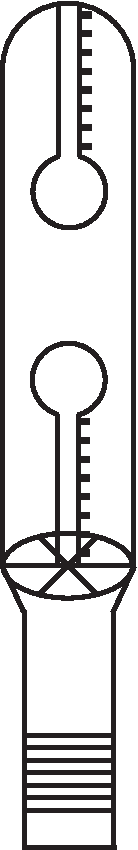
\includegraphics[width=0.1\textwidth]{images/35_14_2_129r}\\\textit{[Fig. 2]}
   %\caption{Bildbeschreibung}
    \end{center}
\pstart \textso{P. 91.}\edtext{}{\lemma{\textso{91.}}\Bfootnote{\cite{00143}\textsc{L. Magalotti}, a.a.O., S.~LXXXXI.}} Experimentum notabile. Inserta sunt vacuo Torricelliano\protect\index{Sachverzeichnis}{vacuum!Torricellianum} (antequam fieret scilicet) duo Thermometra\protect\index{Sachverzeichnis}{thermometrum} exigua clausa alterum in summo alterum in imo vacui. Hoc facto duae pilae\protect\index{Sachverzeichnis}{pila} ex ferro\protect\index{Sachverzeichnis}{ferrum} candenti appropinquentur ut calorem\protect\index{Sachverzeichnis}{calor} dent.  Alterum autem Thermometrum\protect\index{Sachverzeichnis}{thermometrum} habeat pilam\protect\index{Sachverzeichnis}{pila} sursum, nempe  id quod inferius alterum pilam\protect\index{Sachverzeichnis}{pila} deorsum nempe id quod superius.  Appropinquent duae istae massae\protect\index{Sachverzeichnis}{massa} ferri\protect\index{Sachverzeichnis}{ferrum} candentis cannae in  distantia aequali, sed inaequali a pilis Thermometrum\protect\index{Sachverzeichnis}{thermometrum}, ita ut  inferiori sit vicinior, ut calor\protect\index{Sachverzeichnis}{calor} qui semper in aere vadit in altum,  aequalius distribuatur. Nos repetitis saepe experimentis, dicere possumus Thermometrum\protect\index{Sachverzeichnis}{thermometrum} superius sentire magis calorem quam inferius, sed quando  canna est aere plena, differentia adhuc major est, aliquando enim pervenit  ad 5 gradus, cum in Vacuo non sit nisi duorum.\pend \clearpage \pstart \textso{P. 93.}\edtext{}{\lemma{\textso{93.}}\Bfootnote{\cite{00143}\textsc{L. Magalotti}, a.a.O., S.~LXXXXIII.}} Si quid in vacuo ope speculi concavi\protect\index{Sachverzeichnis}{speculum!concavum} vellentis\protect\index{Sachverzeichnis}{lens} accendatur, fumus in eo descendit. Ergo non ascendit in aere nisi quia aer levior.\pend 
\pstart \textso{P. 96.} De sono\protect\index{Sachverzeichnis}{sonus} ajunt \selectlanguage{italian}\textit{un sonaglio suona nel  voto come nell'aria.}\selectlanguage{latin}\edtext{}{\lemma{\textit{nell'aria.}}\Bfootnote{\cite{00143}\textsc{L. Magalotti}, a.a.O., S.~LXXXXVI.}} \selectlanguage{italian}\textit{Et suono dell'organetto invariato nell'aria rara, nella naturale, e nell'artifizialmente compressa.}\selectlanguage{latin}\edtext{}{\lemma{\textit{compressa.}}\Bfootnote{\cite{00143}\textsc{L. Magalotti}, a.a.O., S.~LXXXXVIII.}}\pend \pstart \textso{P. 100}\edtext{}{\lemma{\textso{100}}\Bfootnote{\cite{00143}\textsc{L. Magalotti}, a.a.O., S.~C.}} Liquida in canalibus angustis assurgunt  ultra libellam in vacuo quoque. Non est ergo hoc ab aeris pressione\protect\index{Sachverzeichnis}{pressio!aeris}.\pend \pstart \textso{P. 108.}\edtext{}{\lemma{\textso{108.}}\Bfootnote{\cite{00143}\textsc{L. Magalotti}, a.a.O., S.~CVIII.}} Aqua naturalis (initio) bullas dat  in vacuo, sed magis aqua tepida, quae ob hanc ebullitionem nihilo refrigeratur. Aqua glacie refrigidata dabat quatuor aut quinque minutissimas  bullas.\pend \pstart \textso{P. 111}.\edtext{}{\lemma{\textso{111.}}\Bfootnote{\cite{00143}\textsc{L. Magalotti}, a.a.O., S.~CXI.}} Nix non liquefit citius in vacuo, quam in aere.\pend \pstart \textso{P. 112.}\edtext{}{\lemma{\textso{112.}}\Bfootnote{\cite{00143}\textsc{L. Magalotti}, a.a.O., S.~CXII.}} Quando Margaritae in aceto\protect\index{Sachverzeichnis}{acetum}  distillato, in vacuo dissolvuntur, formantur bullae ad margaritas, quae assurgentes ad superficiem ita fortiter adhaerent Margaritas, ut eas serum usque ad aceti\protect\index{Sachverzeichnis}{acetum} superficiem elevent,  quo facto evanescentibus bullis, Margaritae recedunt, donec continuata solutione  a novis bullis redeleventur.\pend \pstart 